\addcontentsline{toc}{subsubsection}{Skálák fokaira épülő hangzatok}
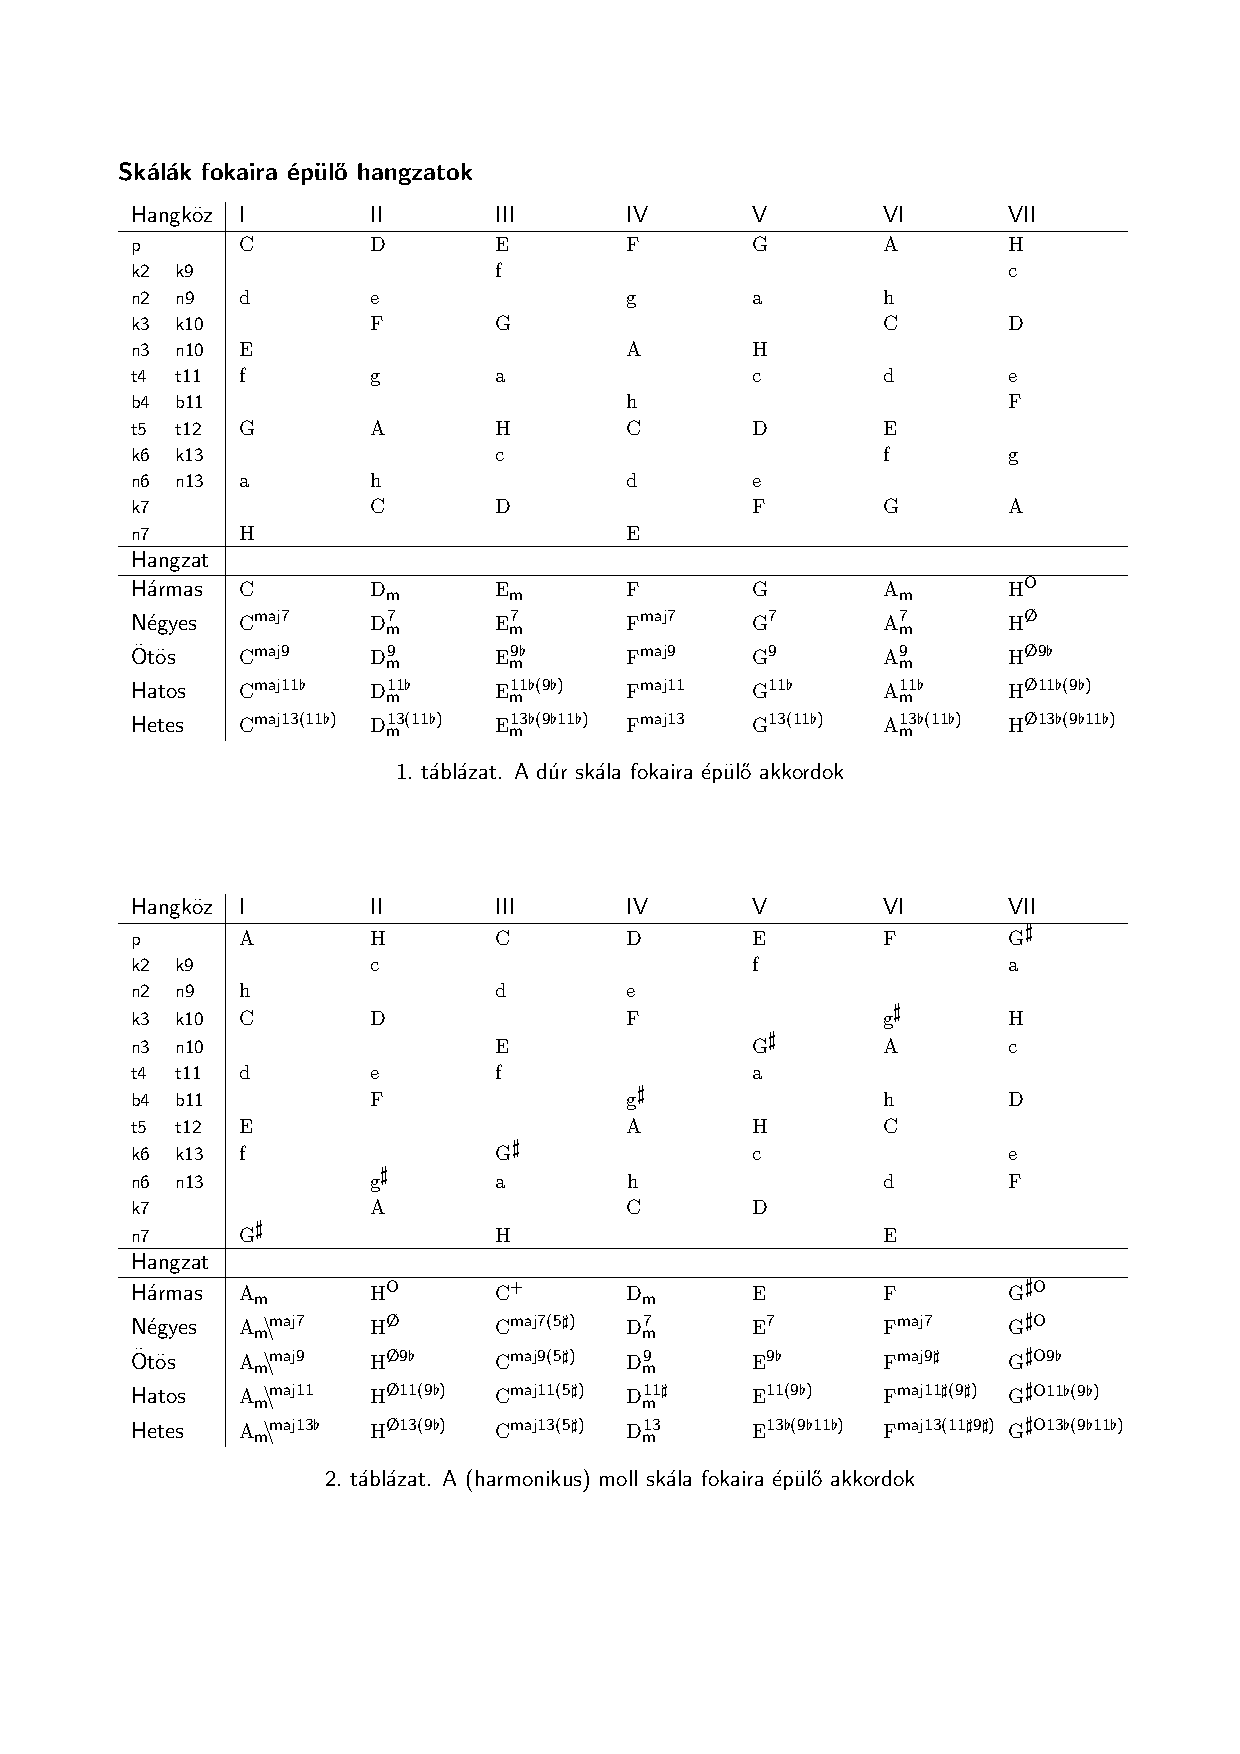
\includepdf[pages=-, pagecommand={\thispagestyle{plain}}]{./appendix/app_scalechords.pdf}

\phantomsection\addcontentsline{toc}{subsection}{Skála minták}
\label{sec:skalamintak}
\addcontentsline{toc}{subsubsection}{Modális skálák}
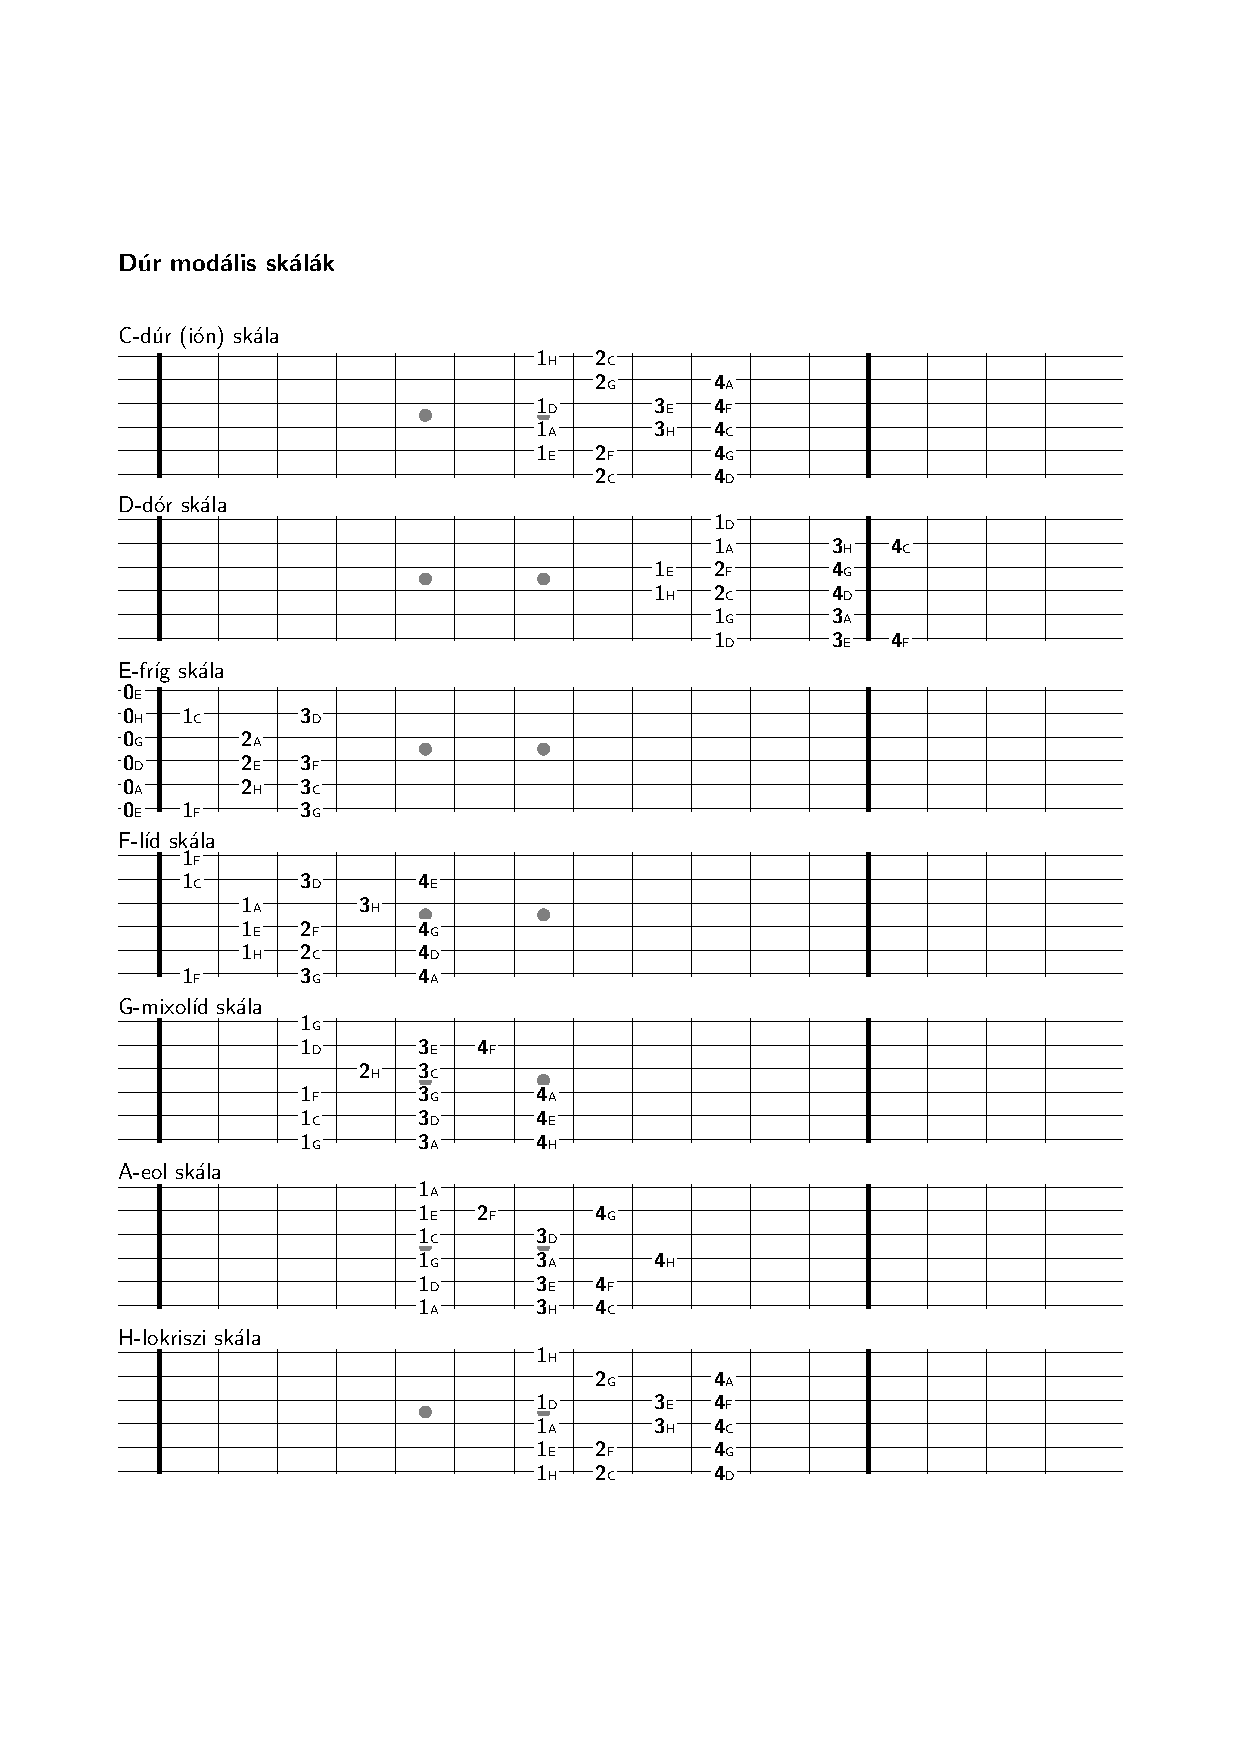
\includepdf[pages=-, pagecommand={\thispagestyle{plain}}]{./appendix/app_modalscales.pdf}
\addcontentsline{toc}{subsubsection}{A harmonikus A-moll skála fokai}
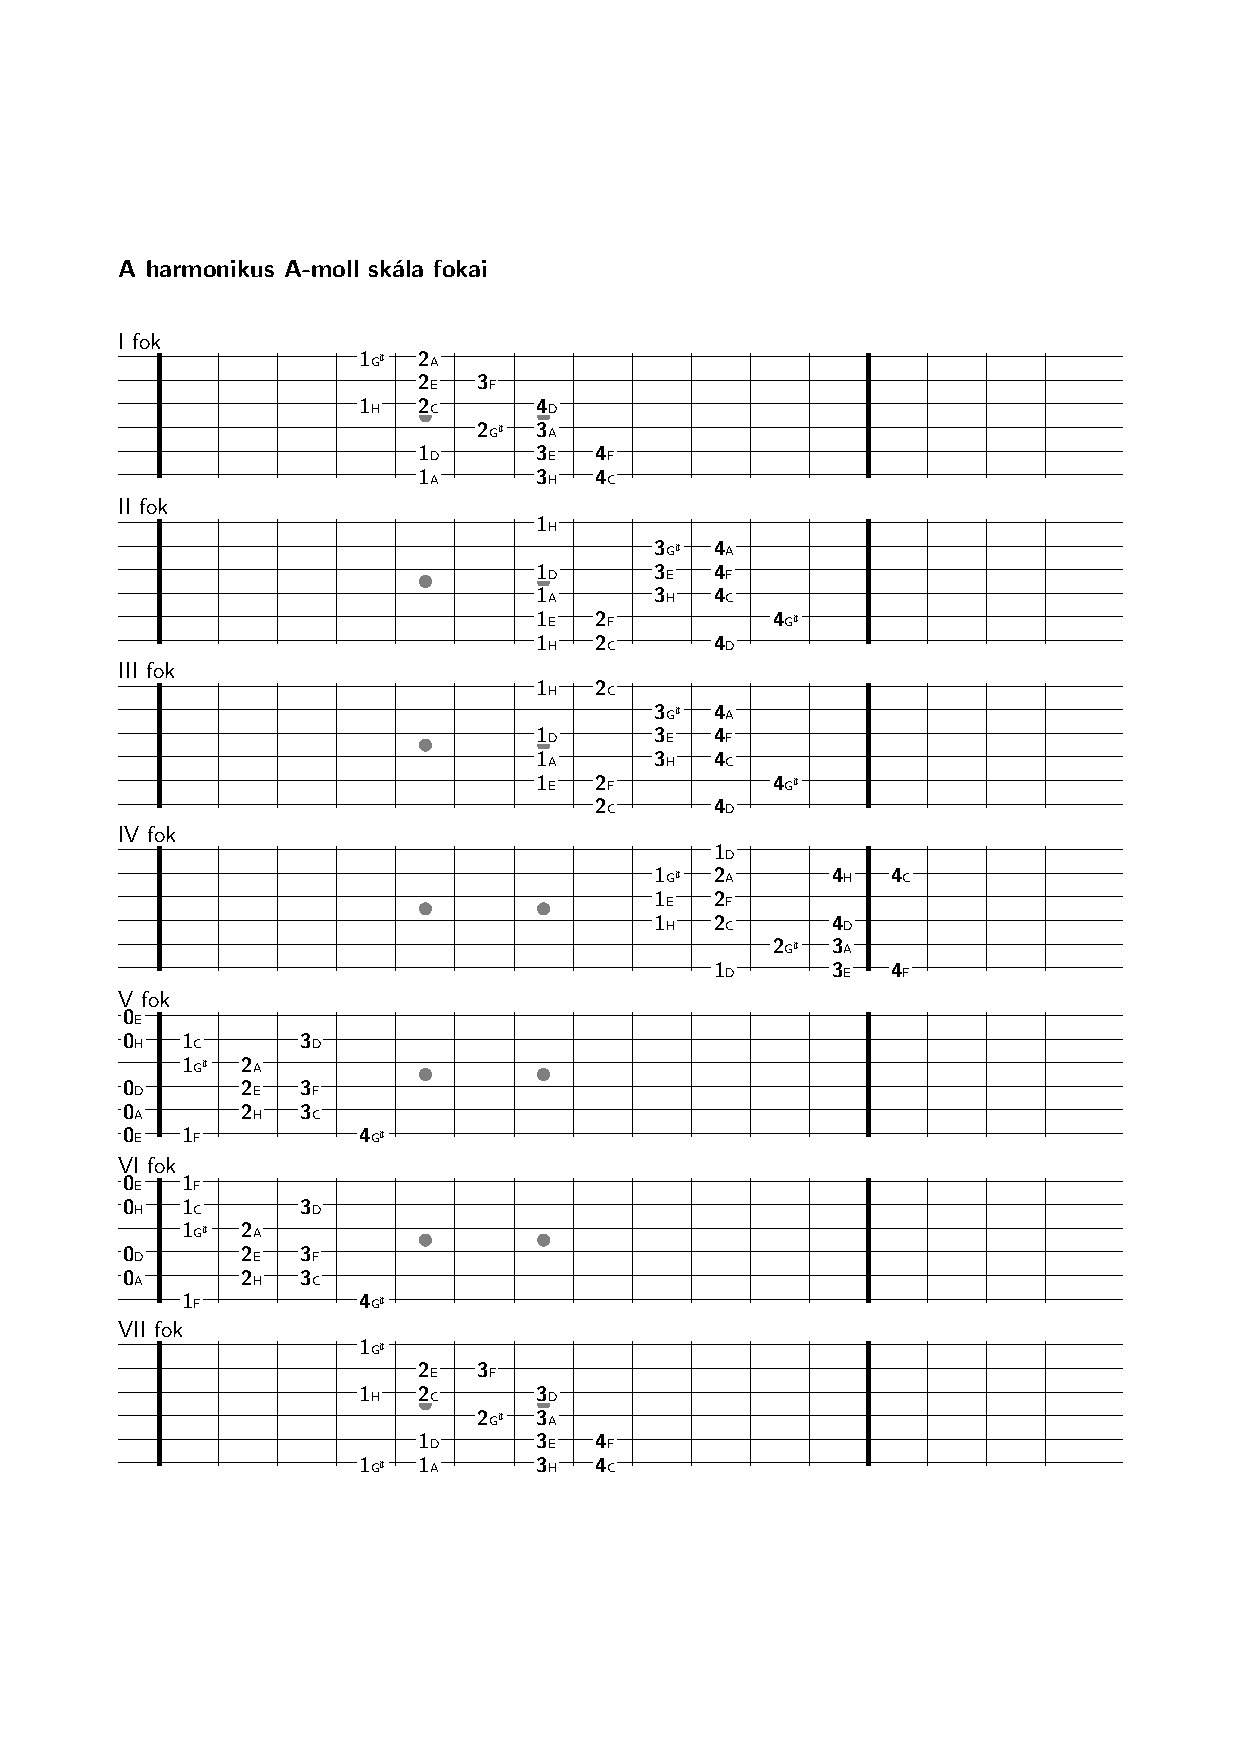
\includepdf[pages=-, pagecommand={\thispagestyle{plain}}]{./appendix/app_mollscales.pdf}
\addcontentsline{toc}{subsubsection}{A melodikus A-moll skála fokai}
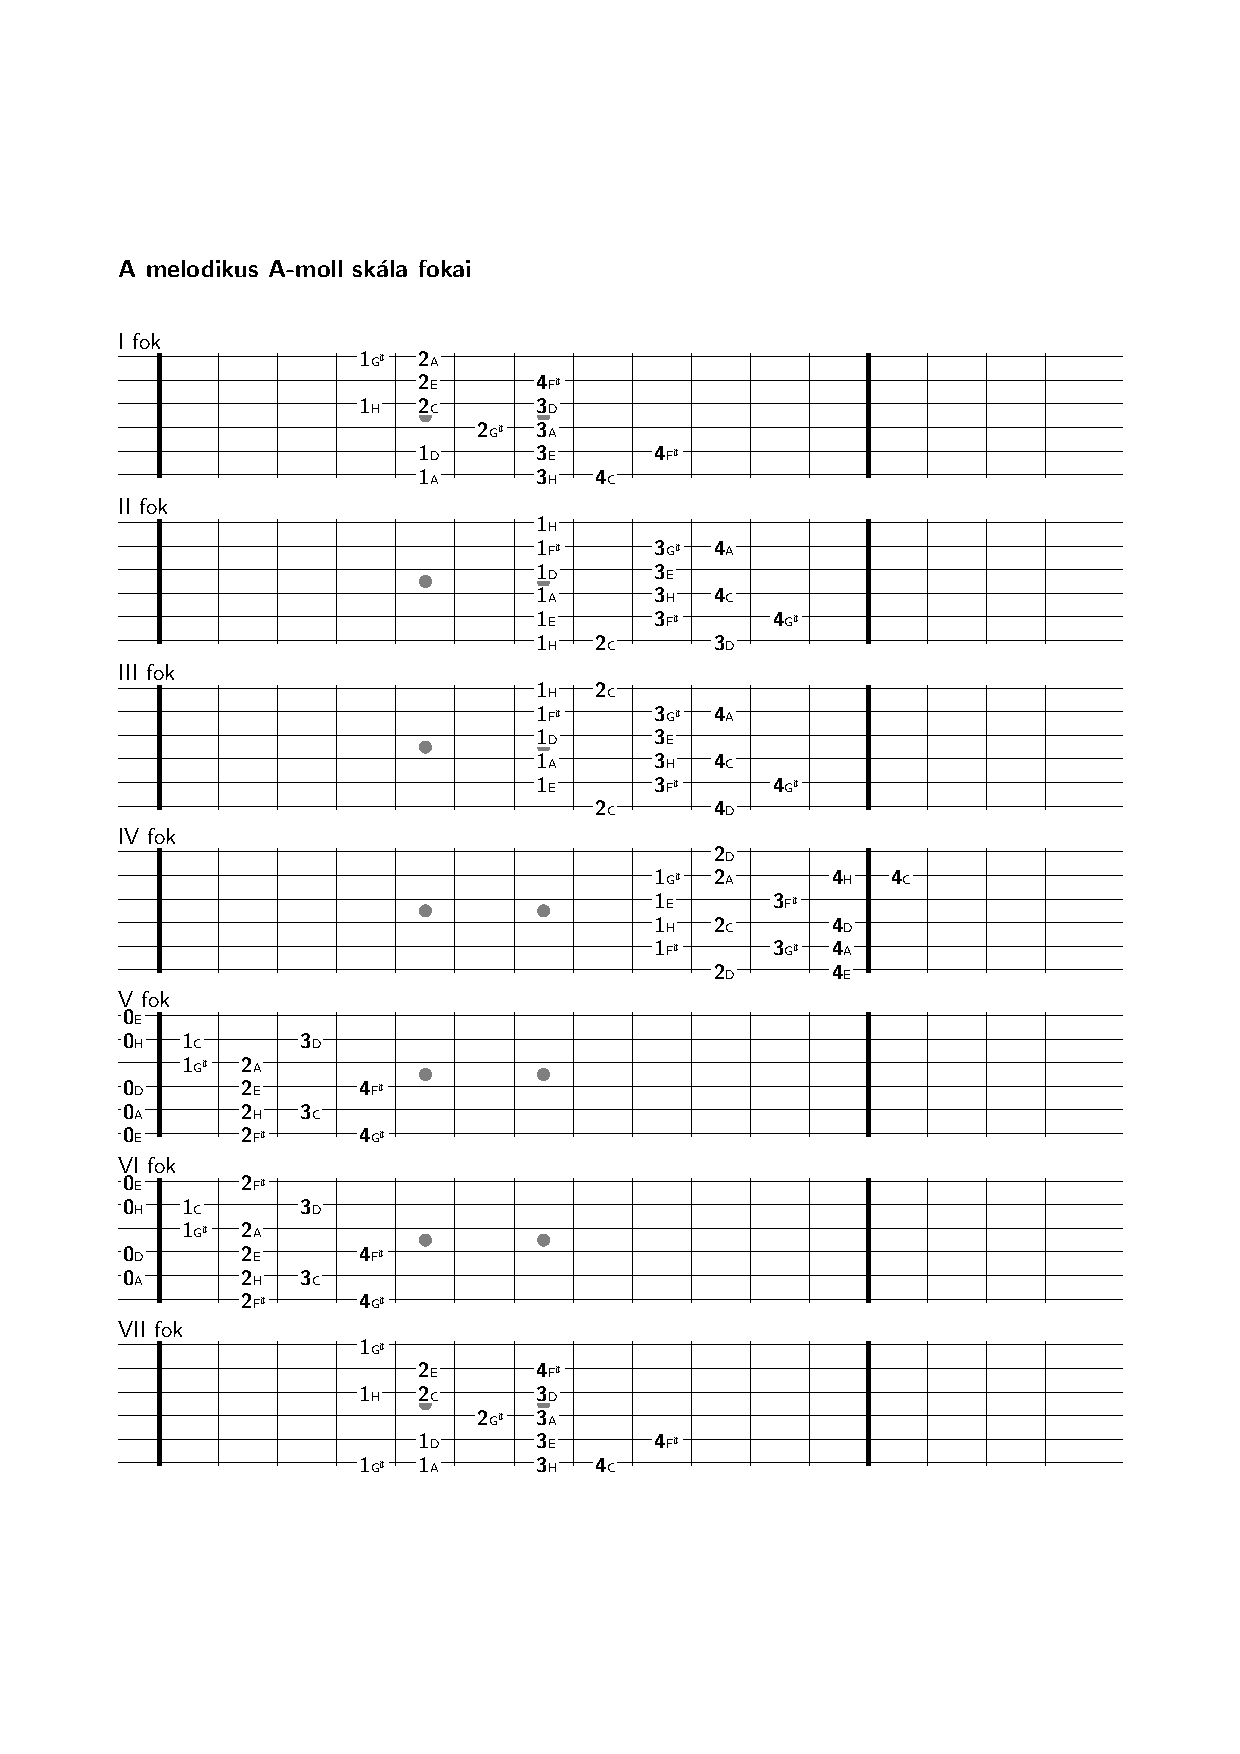
\includepdf[pages=-, pagecommand={\thispagestyle{plain}}]{./appendix/app_mmollscales.pdf}
\addcontentsline{toc}{subsubsection}{Speciális skálák}
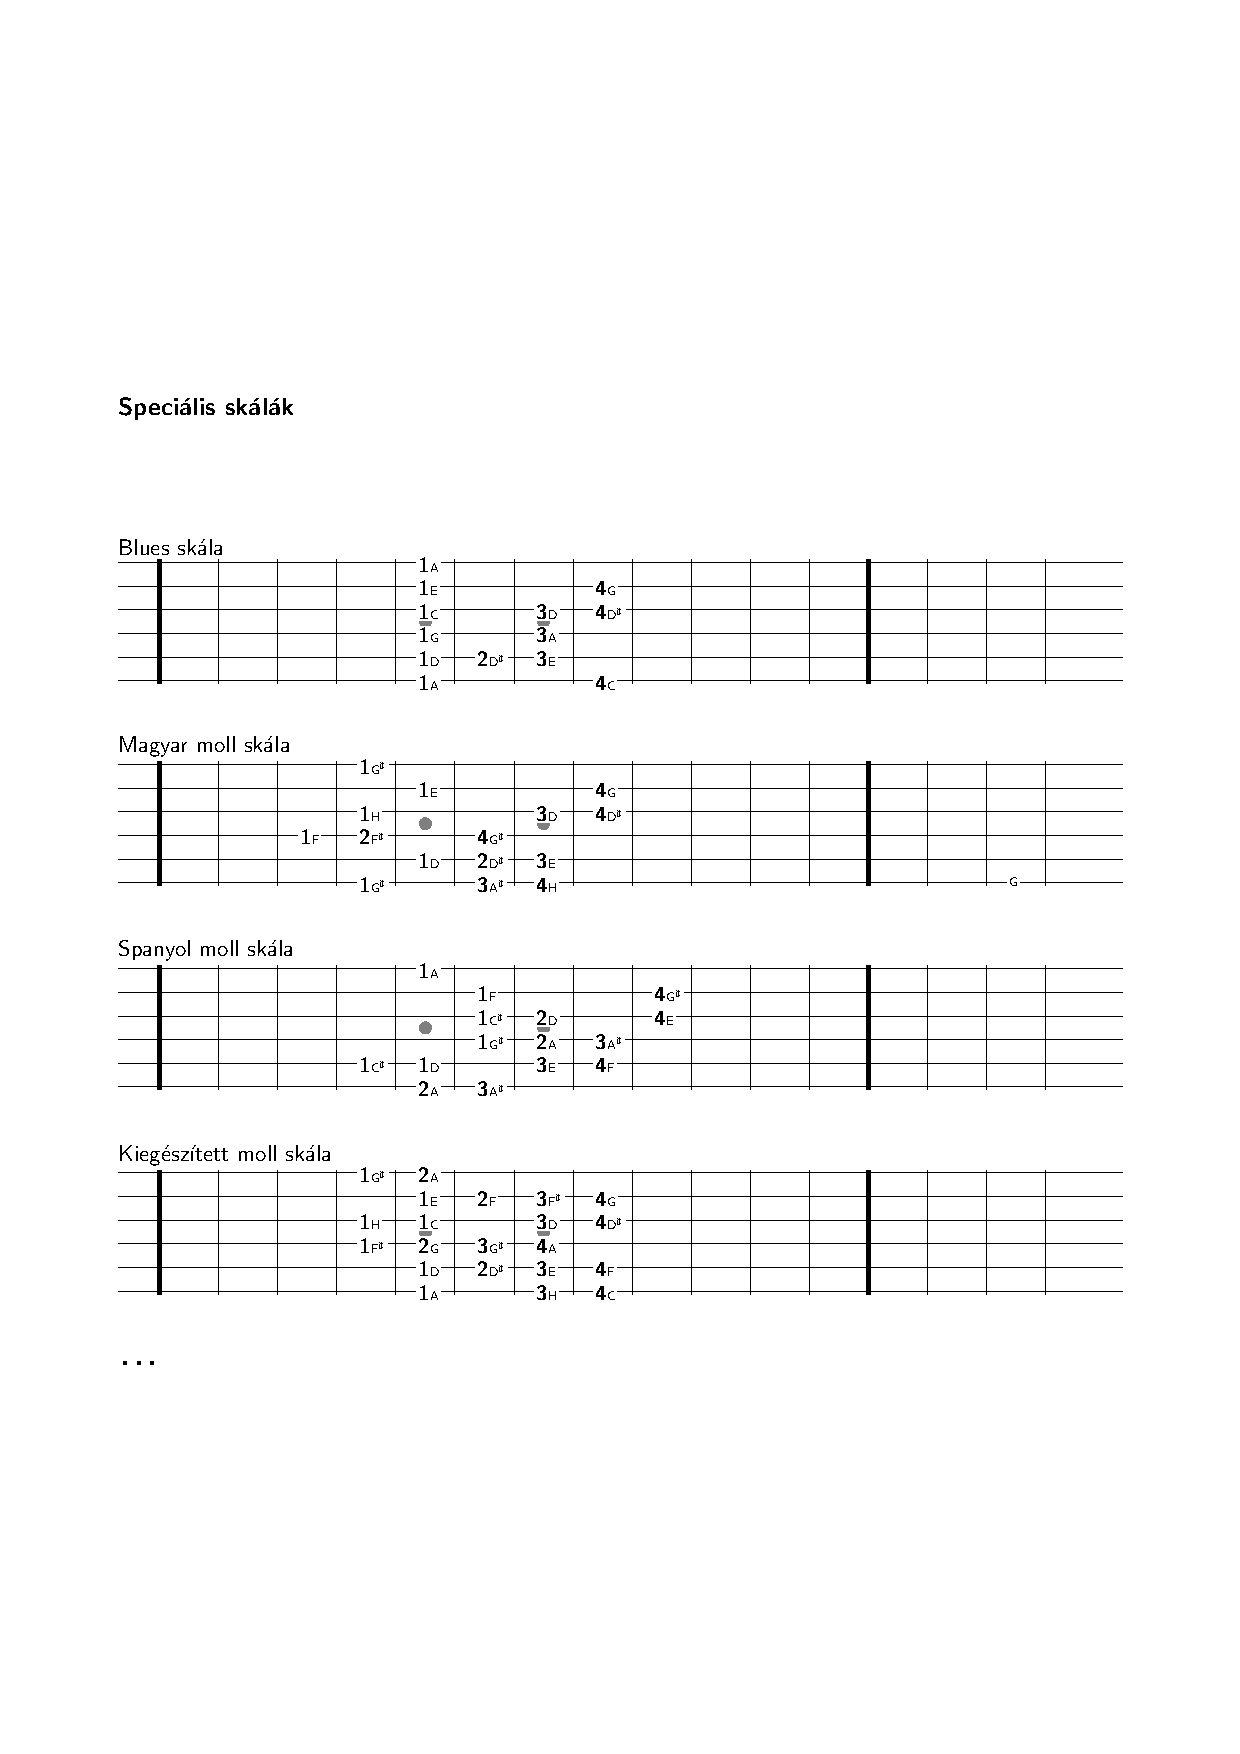
\includepdf[pages=-, pagecommand={\thispagestyle{plain}}]{./appendix/app_specscales.pdf}

\addcontentsline{toc}{subsection}{Az akkordok felépítése}
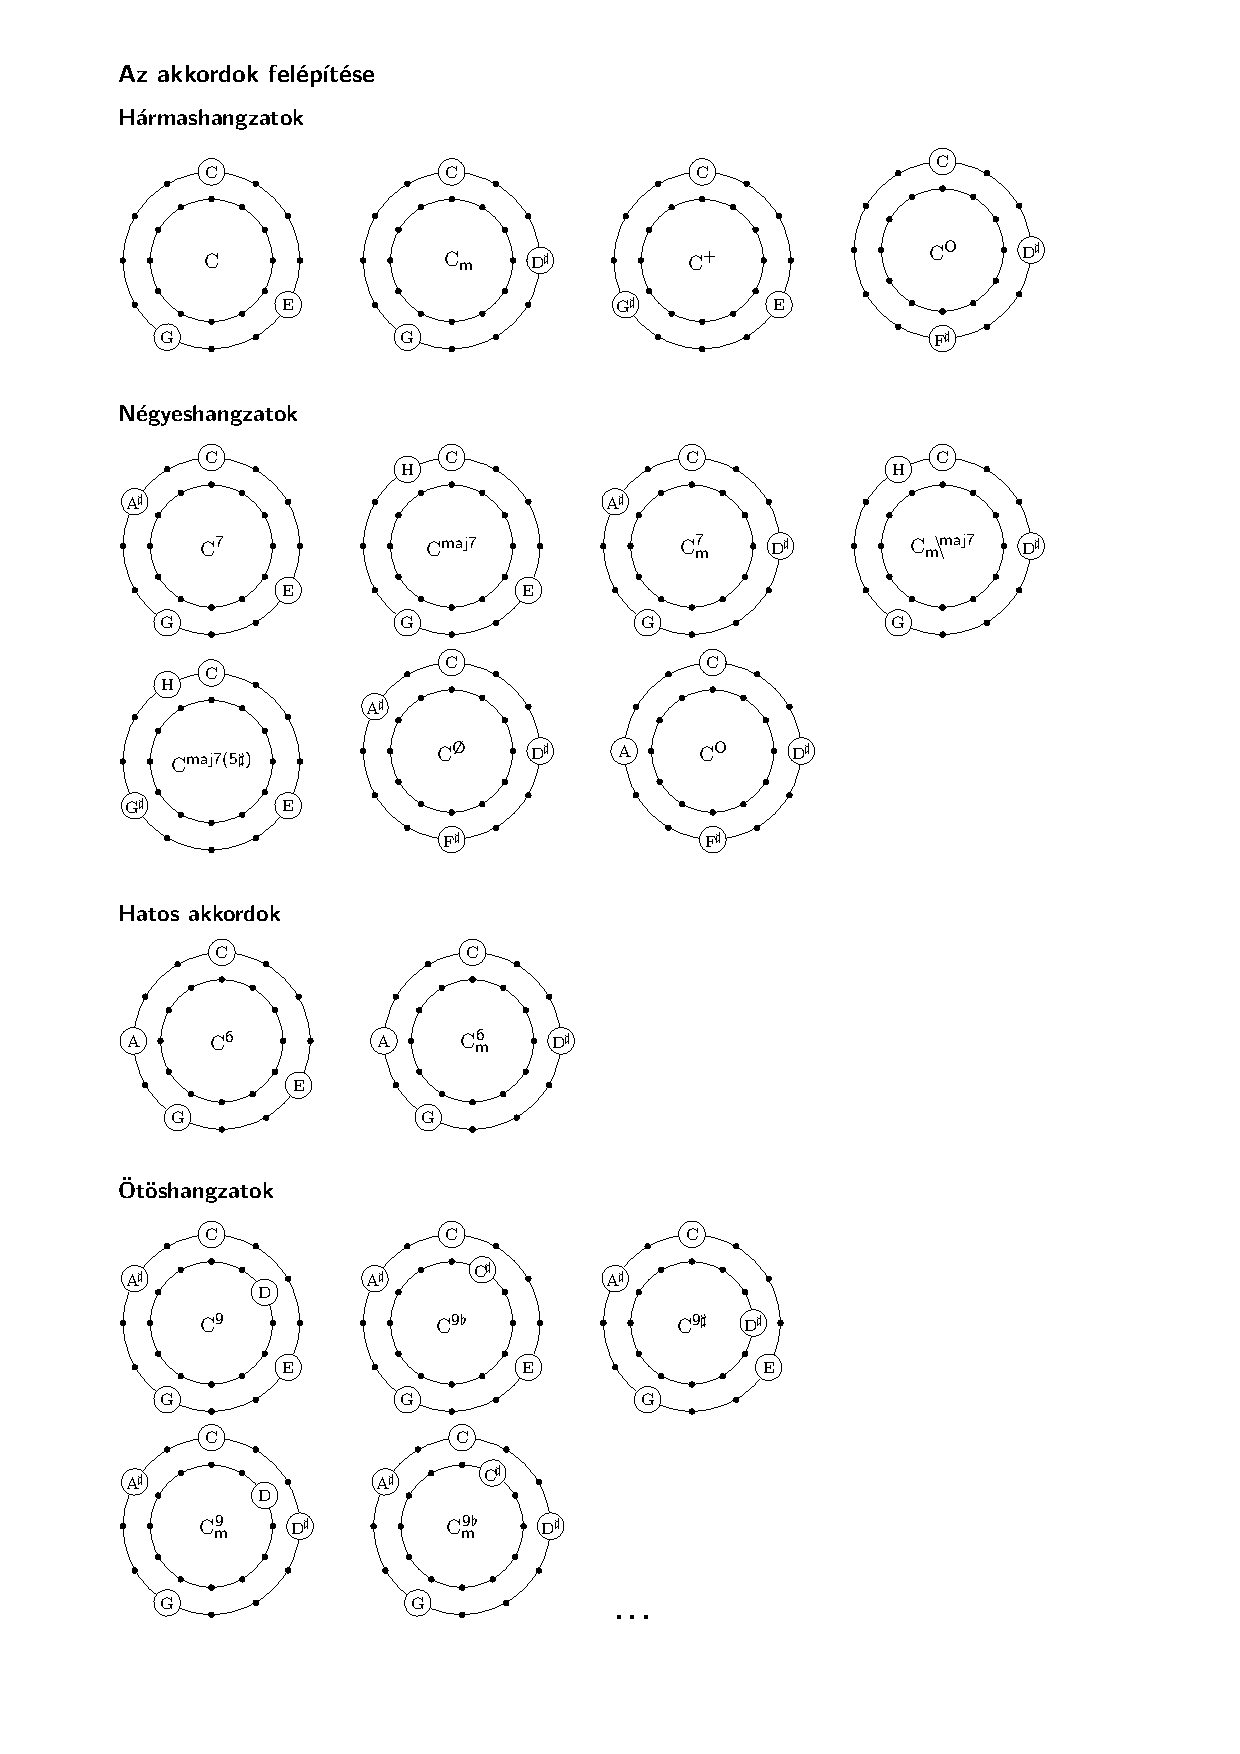
\includepdf[pages=-, pagecommand={\thispagestyle{plain}}]{./appendix/app_chordstructure.pdf}

\phantomsection\addcontentsline{toc}{subsection}{Akkord minták}
\phantomsection\addcontentsline{toc}{subsubsection}{Hármashangzatok}
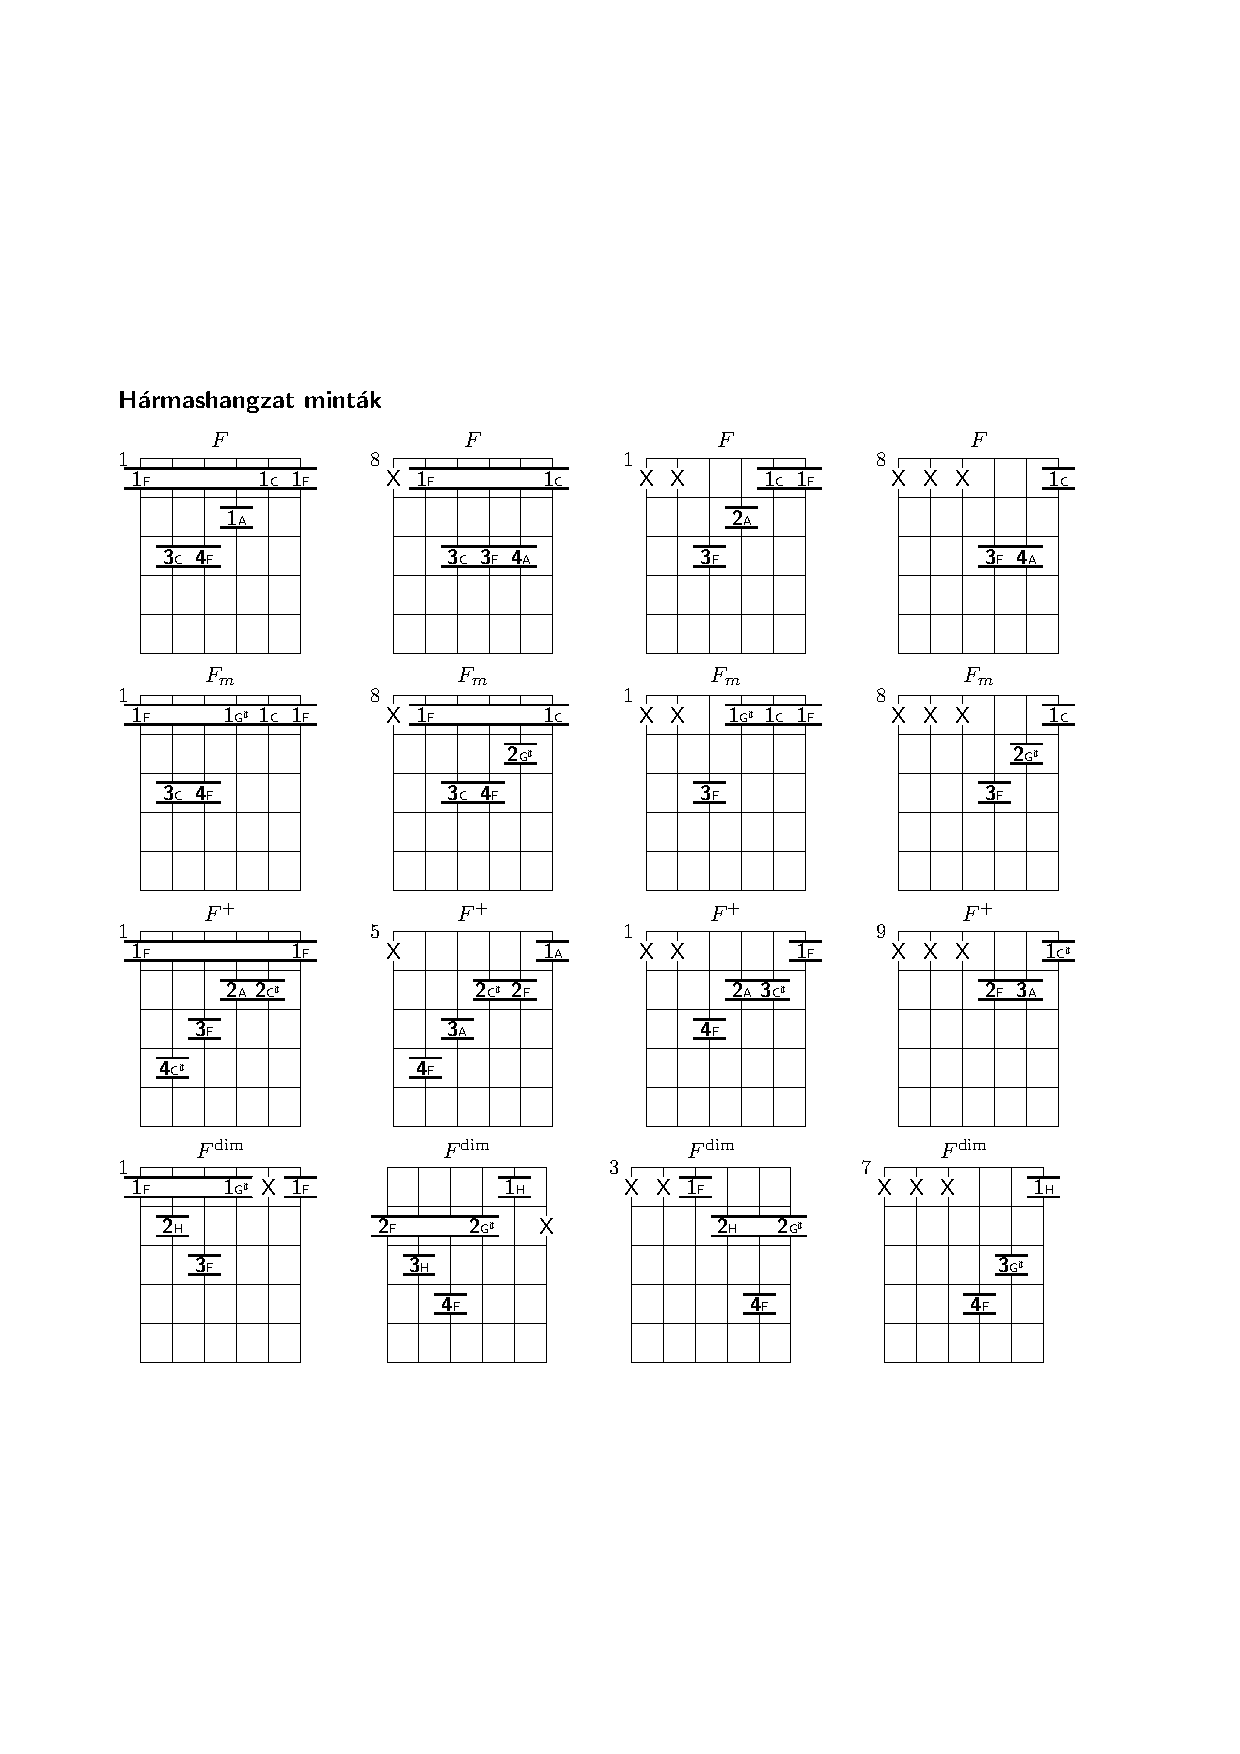
\includepdf[pages=-,pagecommand=\thispagestyle{plain}]{./appendix/app_chord3.pdf}
\phantomsection\addcontentsline{toc}{subsubsection}{Négyeshangzatok}
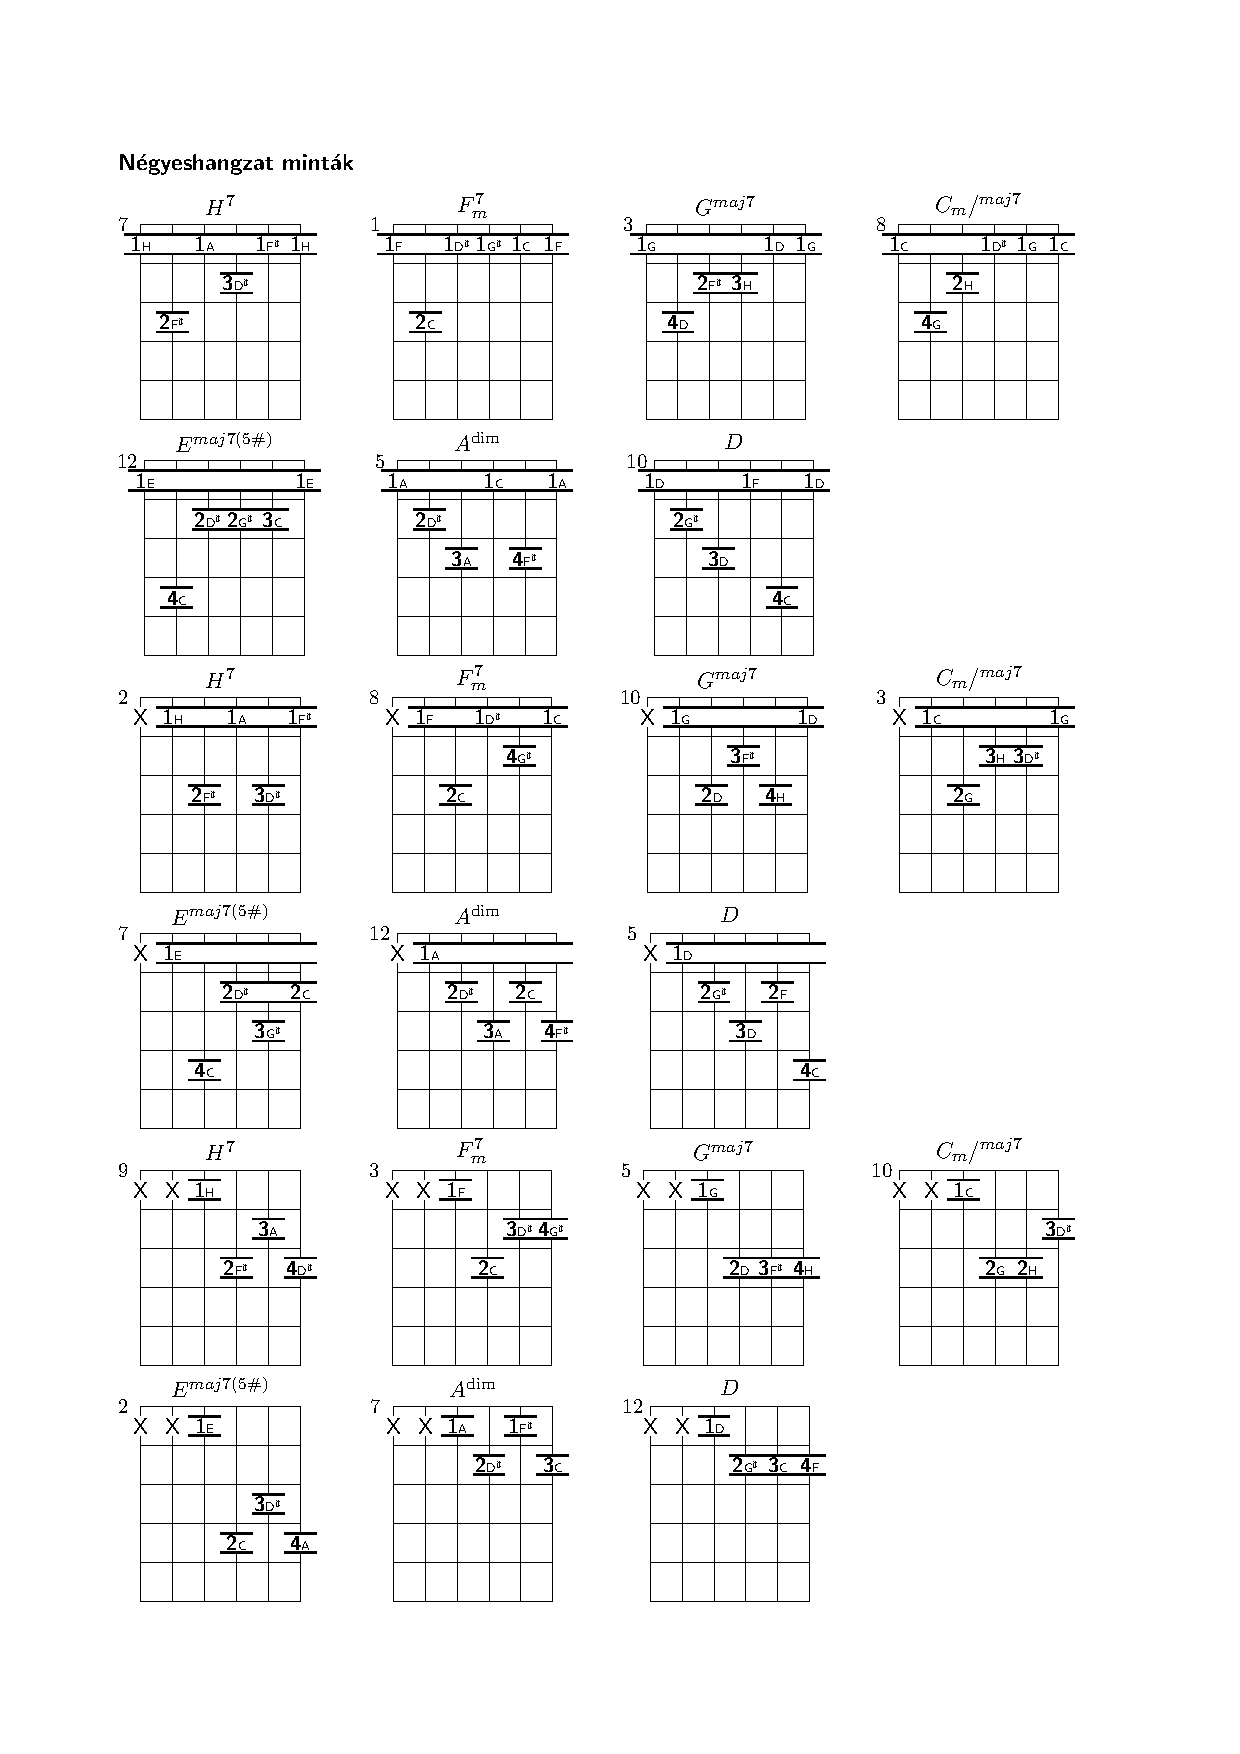
\includepdf[pages=-,pagecommand=\thispagestyle{plain}]{./appendix/app_chord4.pdf}

\phantomsection\addcontentsline{toc}{subsection}{Kották}
\phantomsection\addcontentsline{toc}{subsubsection}{Capriccio}
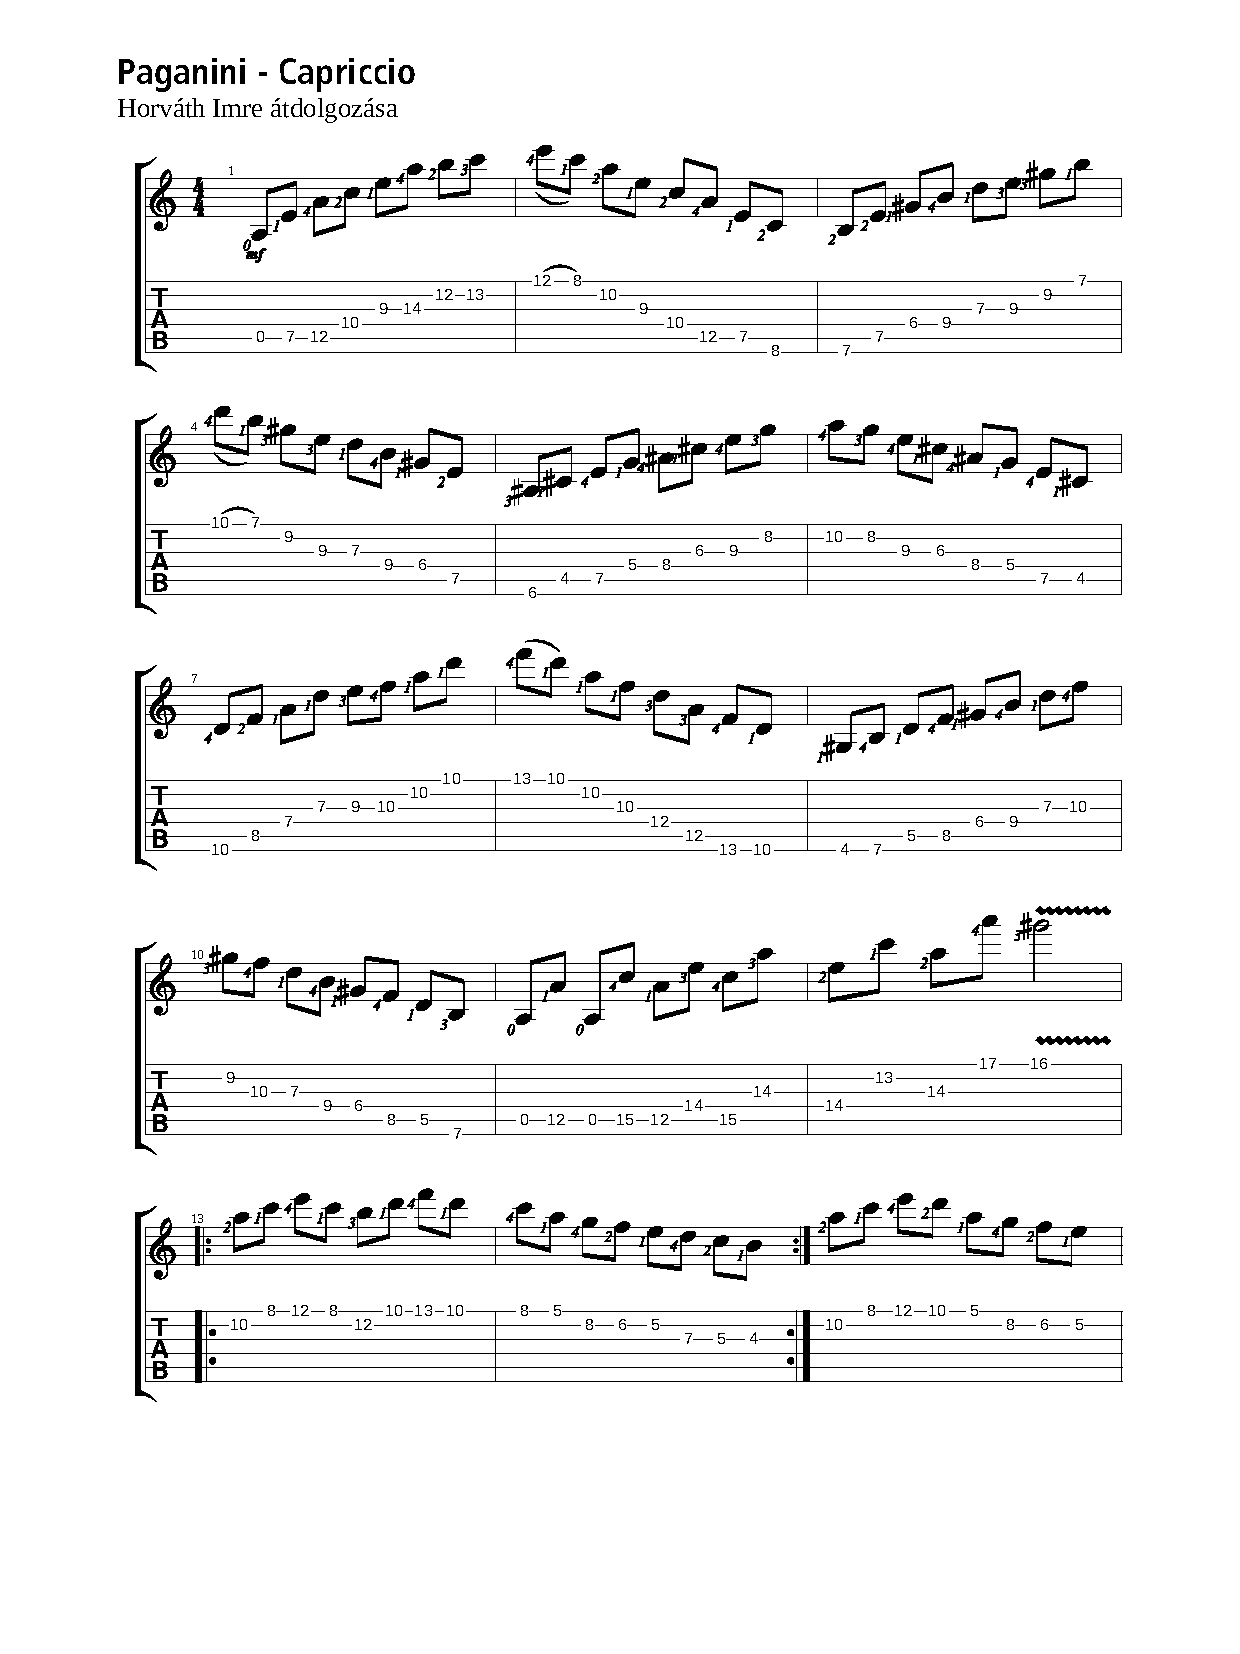
\includepdf[pages=-,pagecommand=\thispagestyle{plain}]{./notes/capriccio.pdf}
\phantomsection\addcontentsline{toc}{subsubsection}{Spanish Romance}
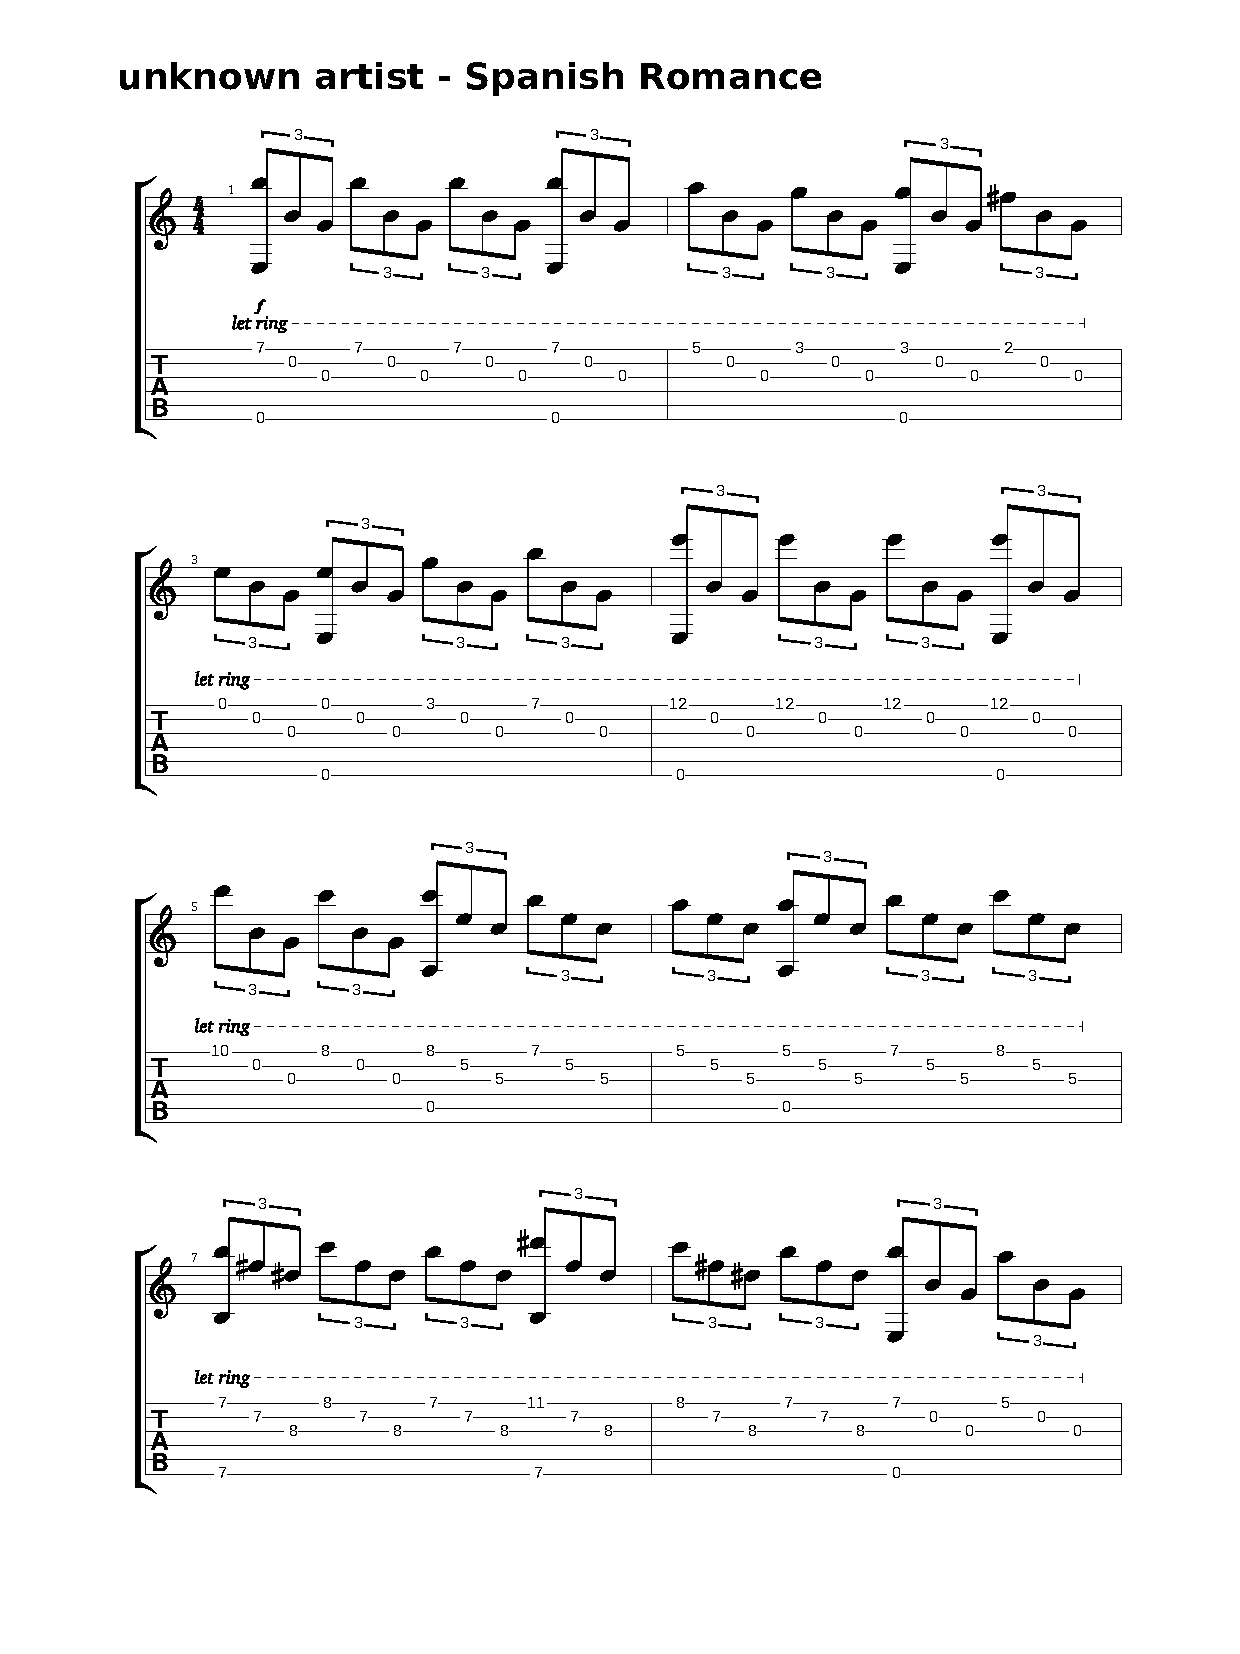
\includepdf[pages=-,pagecommand=\thispagestyle{plain}]{./notes/spanishromance.pdf}
\phantomsection\addcontentsline{toc}{subsubsection}{Is There Anybody Out There?}
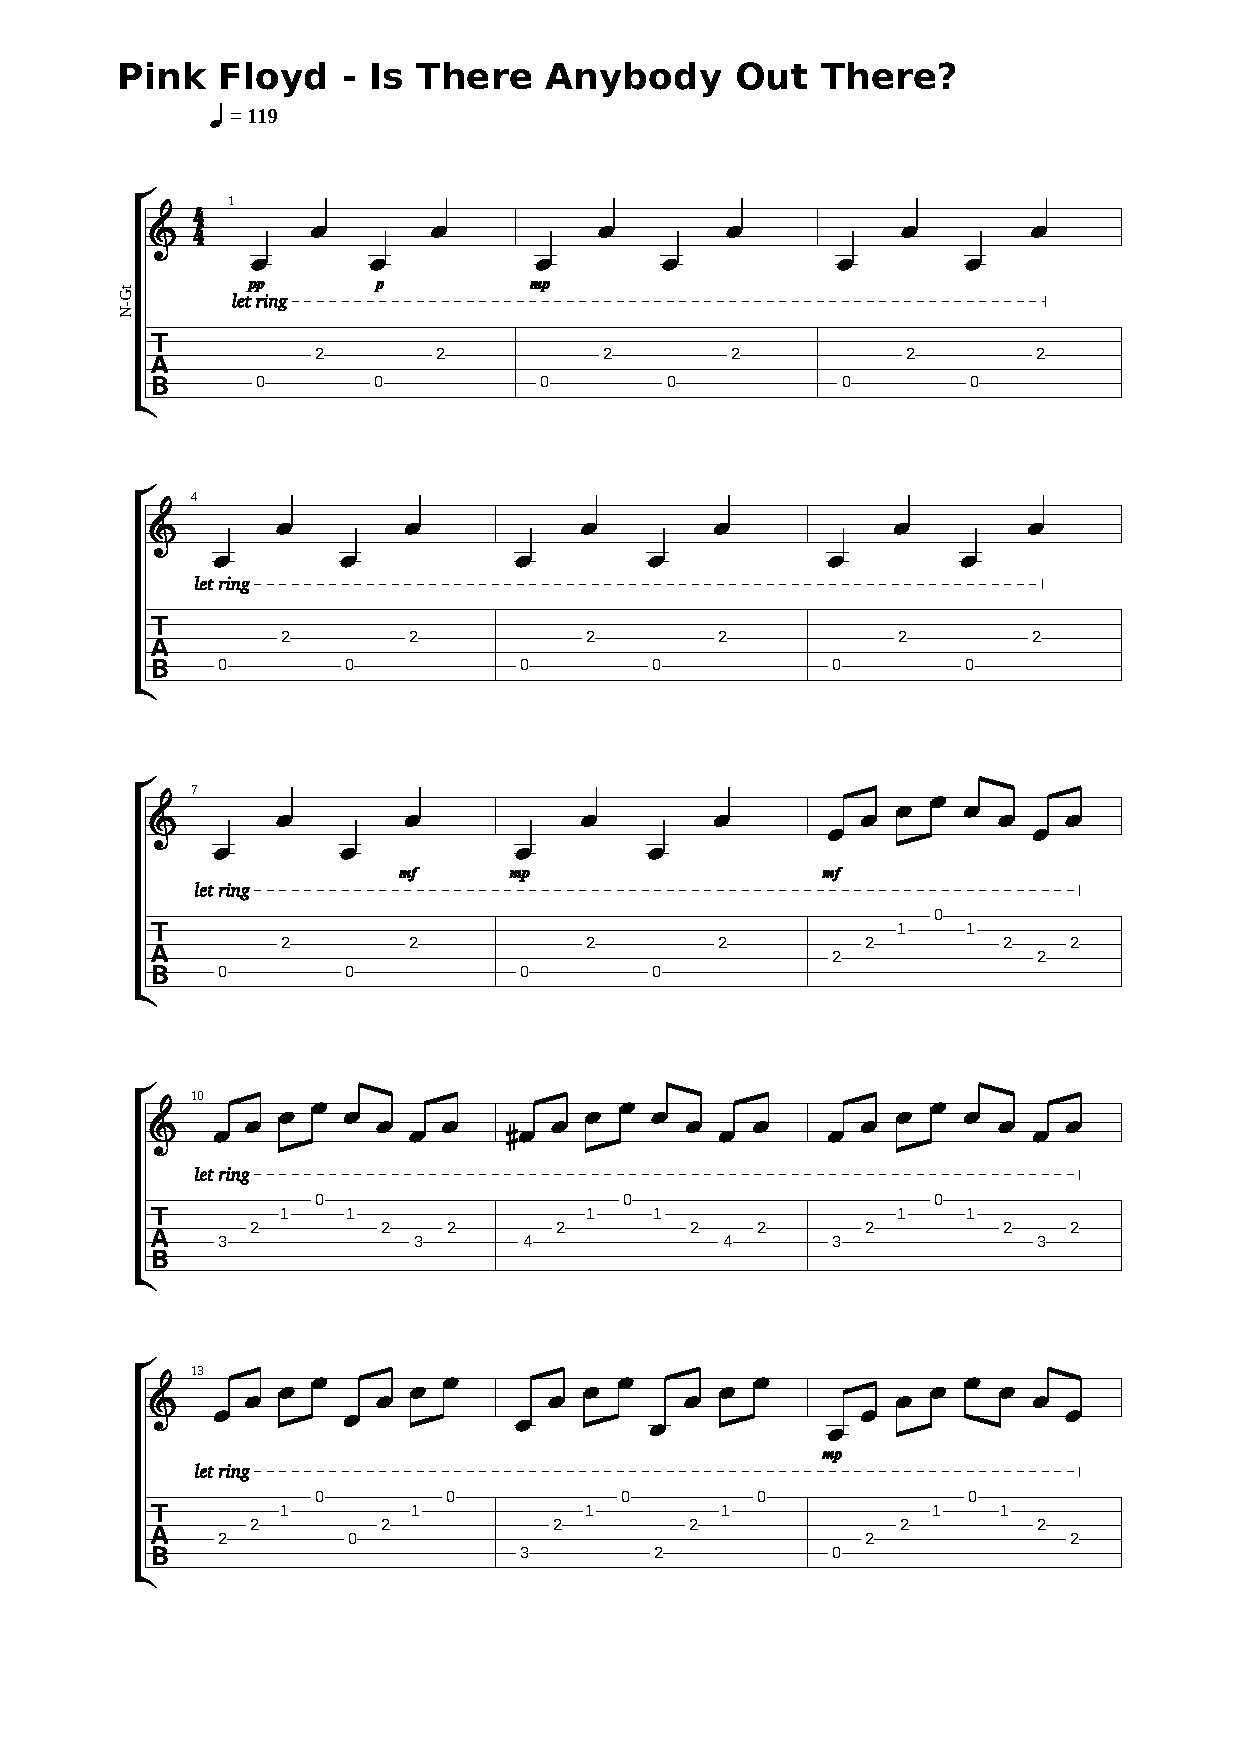
\includepdf[pages=-,pagecommand=\thispagestyle{plain}]{./notes/isthereanybodyoutthere.pdf}

